\documentclass{article}
\usepackage[utf8]{inputenc}
\usepackage{graphicx}
\usepackage{amsmath}
\title{NP-Complete graph problems - KombSøg 2017}
        \author{Anders H Pedersen }
        \date{May 2017}
\begin{document}

\maketitle

\begin{center}
\textit{The graph problems and reductions below were introduced by Thomas Dueholm Hansen, at the lecture on NP-Complete graph problems may 3 2017.}
\end{center}

\section{Graph problems}
\subsection{INDEPENDENT SET}
\textbf{Given:} Graph G = (V,E), target K. \\
\textbf{Question:} Does there exist $I \subseteq V$ such that $|I| \geq K$\\ and for all $u,v\in I$ we have $(u,v) \notin E$? 
\subsection{CLIQUE}
\textbf{Given:} Graph G = (V,E), target K. \\
\textbf{Question:} Does there exist $C \subseteq V$ such that $|C| \geq K$\\ and for all $u,v\in C$ we have $(u,v) \in E$?
\subsection{VERTEX COVER}
\textbf{Given:} Graph G = (V,E), budget B. \\
\textbf{Question:} Does there exist $C \subseteq V$ such that $|C| \leq B$\\
and for all $(u,v) \in E$ we have $(u \in C \lor v \in C)$?
\subsection{MAX CUT}
\textbf{Given:} Graph G = (V,E), target K. \\
\textbf{Question:} Does there exist a cut  $(S,V\setminus S)$ of size at least K?\\
\subsection{MAX BISECTION}
\textbf{Given:} Graph G = (V,E), target K.\\
\textbf{Question:} Does there exist a cut  $(S,V\setminus S)$ of size at least K, such that $|S| =  |V \setminus S|$?
\subsection{BISECTION WIDTH}
\textbf{Given:} Graph G = (V,E), target K.\\
\textbf{Question:} Does there exist a cut  $(S,V\setminus S)$ of size at most K, such that $|S| =  |V \setminus S|$?
\subsection{HAMILTONIAN PATH}
\textbf{Given:} Graph G = (V,E).\\
\textbf{Question:} Does G have a path that visits every vertex exactly once?\\
\subsection{TSP}
\textbf{Given:} Distance matrix D, target t. \\
\textbf{Question:} Is there a tour of length at most t that visits every node in the graph defined by D exactly once?\\
\section{Reductions}
As always, in a reduction $L_1 \le L_2$, we describe a polynomial time computable function r, such that $\forall x: x\in L_1 \iff r(x) \in L_2$. We then argue that it is indeed polynomial, and that both directions of the bi-implication holds.\\\\
\subsection{3SAT $\le$ INDEPENDENT SET}
We prove \textbf{Theorem 9.4: INDEPENDENT SET is NP-Complete}, by reducing from 3SAT, which we know is NP-Complete.\\\\
For this reduction we need a gadget, the triangle. The logic behind this is that, if a graph contains a triangle, then at most one of the nodes can be in the independent set. We restrict the class of graphs we consider, to graphs whose nodes can be partitioned in m disjoint triangles. This ensures that an independent set can contain at most m nodes. \\

For each of the m clauses in our input CNF formula, we create a triangle where the nodes are labeled with the literals of the clause. Next, we add an edge between two nodes in different triangles if and only if the nodes correspond to opposite literals. Adding these edges between opposite literals, ensures that we cannot pick both (as it would not be an independent set). The reduction is completed by setting the independent set goal K = m. \\\\\\
\textbf{Example:}\\\\
Given a 3CNF formula:  $f =  (x_1 \lor x_2 \lor x_3) \land (\lnot x_1 \lor \lnot x_2 \lor \lnot x_3) \land (\lnot x_1 \lor x_2 \lor x_3)$\\
We construct the graph shown in figure 1. \\
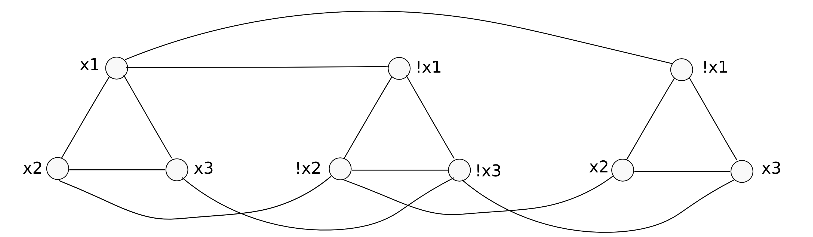
\includegraphics[scale=0.5]{independentset}
\textbf{Figure 1:} Graph r(f) corresponding to the formula f\\\\\\
\textbf{Analysis}\\
For each clause, we just create a triangle. Then we add at most $3 * (m-1)$ edges between the triangles - so the reduction is clearly polynomial.
\\\\
$\implies$ :\\ Given a satisfying assignment for the CNF formula f from above, we must show that the graph, r(f), has an indenpendent set of size K=m. The assignment: $x_1 = 0, x_2 = 1, x_3 = 0$ satisfies the formula, and for our indenpendent set of size K, we pick a node in each triangle which make the corresponding clause true. For the truth assignment we chose above, this means $x_2$ from triangle 1, $\lnot x_1$ in triangle 2, $\lnot x_1$ in triangle 3. (Note that this is not the only valid set since some clauses are satisfied by more than one literals).
\\\\
$\impliedby$ :\\ Given an independent set of size K of r(f), we need to show that there is a satisfying assignment for f. Since it is of size K, it must have one vertex from each triangle, and it cannot contain a variable and its negation. Now, for each vertex in the independent set, we look at the label and assign a truth value to the corresponding variable, so the literal of the label become true. If a variable is not restricted to a truth value by any vertex label, we just assign it some value, since all clauses are already satisfied by the assignments to the other variables.\\\\\\
\textit{Read more in papadimitriou page 188-190.}
\newpage
\subsection{INDEPENDENT SET $\le$ CLIQUE}
The independent set problem asks for a set of vertices of size K. So does the CLIQUE problem. While the independent set problem asks for a set S of vertices where there is no edge between any pair $u,v \in S$.
\\\\\\
\textit{Read more in papadimitriou page 190.}
\subsection{INDEPENDENT SET $\le$ VERTEX COVER}
\subsection{NAESAT $\le$ MAX CUT}
\subsection{3SAT $\le$ HAMILTONIAN PATH}
\subsection{HAMILTONIAN PATH $\le$ TSP}



\end{document}
